To enrich our decision-making model, we introduce four fuzzy attributes. These attributes evaluate the temporal distribution of interventions based on their size, risk, spatial proximity to each other, and environmental sensitivity. They are built upon the principles of fuzzy logic to translate crisp, quantitative data into a more expressive, linguistic framework suitable for multi-criteria analysis.\\

Our methodology for constructing these attributes follows a three-stage process. Crisp numerical data from each intervention is transformed into fuzzy sets over the intervention space, which represent the extent to which an intervention possesses a certain qualitative (linguistic) property. Second, for any given solution, 
we take the fuzzy subset of active interventions in each day and aggregate (add\footnote{Adding the memberships of a fuzzy set is equivalent to computing the cardinality of that fuzzy set.}) these memberships into a "daily mass". This time series quantifies the total presence of that fuzzy property among the interventions active on each day of the planning horizon. Finally, we evaluate the temporal uniformity of this mass distribution using a scalar score derived from Shannon's entropy, allowing for a concise comparison between different solutions.\\

The initial stage, fuzzification, is achieved through one of two methods depending on the nature of the attribute. For properties based on distance, we define a \textbf{linguistic variable}. In this case, the linguistic variable \textit{Distance} defines 5 linguistic terms (close, mid-close, mid, mid-far, far), which are defined over a numerical base variable (distance in meters). The meaning of each linguistic term is captured by a membership function, $\mu(x)$, which assigns a compatibility degree in $[0, 1]$ to each value of the base variable. This degree of compatibility is conceptually distinct from probability, as it is not a frequency of any event. The membership functions the five terms are specified by trapezoidal and triangular numbers as shown in Figure~\ref{fig:fuzzy_distance}. Therefore, 5 values need to be chosen by the decision maker, which specify the boundaries of each fuzzy number.\\


\begin{figure}[!ht]
    \centering
    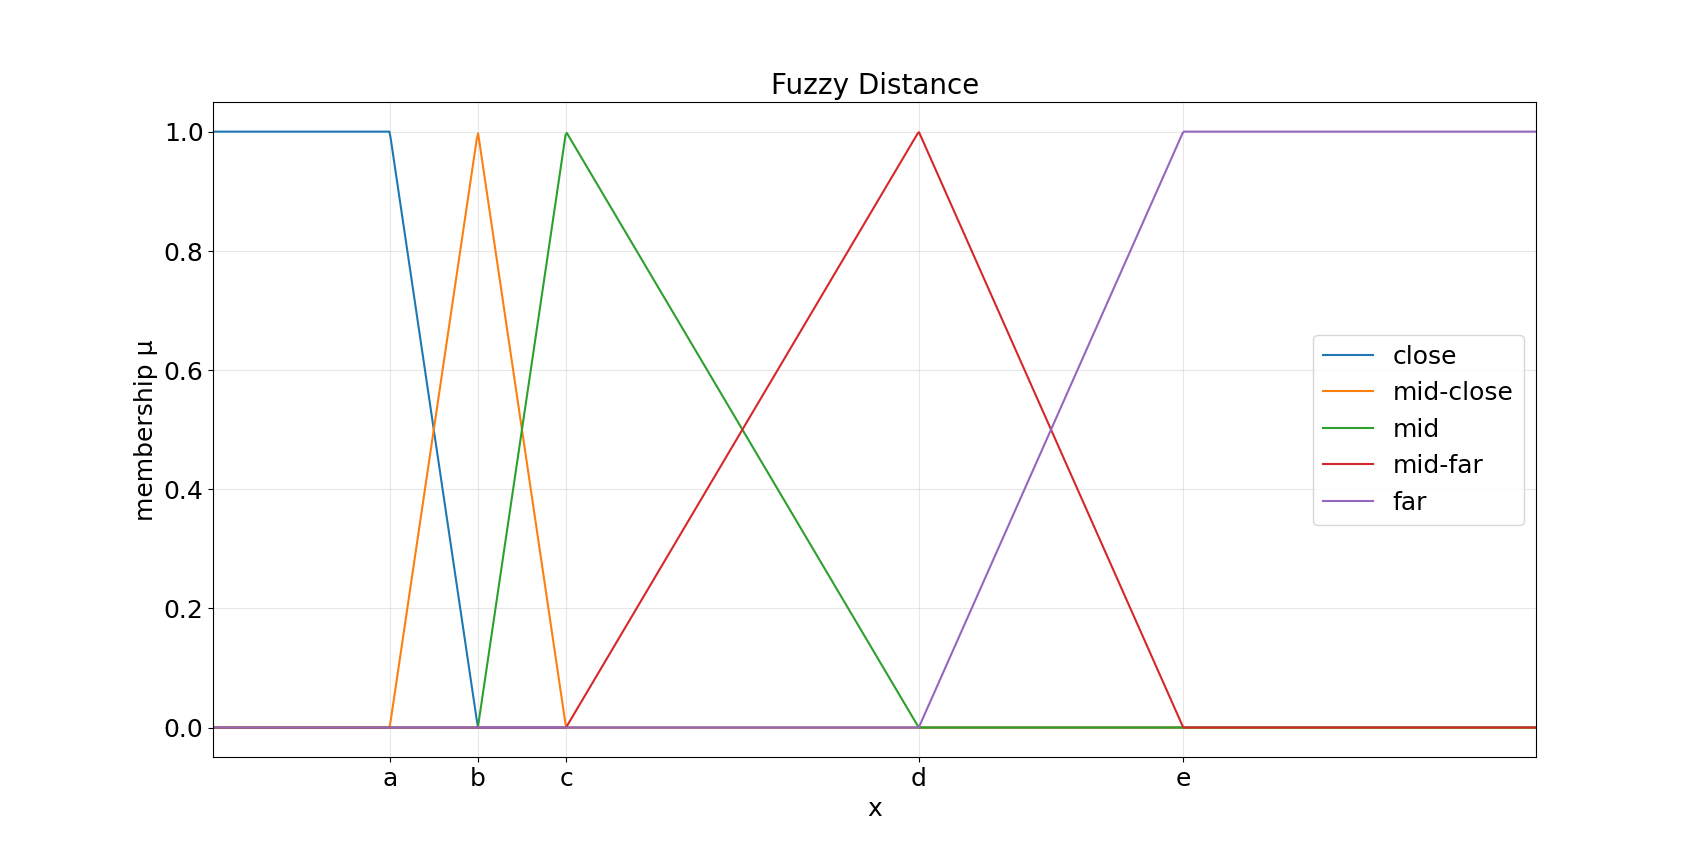
\includegraphics[width=\linewidth]{ch3/figures/Fuzzy distance.png}
    \caption{Fuzzy distance linguistic variable with close, mid-close, mid, mid-far and far membership functions. Five values (a,b,c,d,e) are required for defining the compatibility functions of the terms: 2 trapezoidal fuzzy numbers for close and far and 3 triangular fuzzy numbers for mid-close, mid and mid-far.}
    \label{fig:fuzzy_distance}
    \end{figure}

For attributes like intervention size and risk, where clear-cut boundaries are harder to set, we employ a data-driven approach using \textbf{fuzzy c-means clustering}. This unsupervised algorithm partitions the set of interventions into a specified number of clusters (in our case, five) based on their data. Unlike hard clustering, it assigns each intervention a membership degree to every cluster, reflecting partial associations. For example, an intervention could be 80\% medium and 20\% mid-large size. We apply this technique to the mean size and mean risk of each intervention, with the resulting cluster centroids, representing the prototypical value for each fuzzy category, shown in Table~\ref{tab:fuzzy_centroids}.

\begin{table}[!ht]
    \centering
    \begin{tabular}{lcc}
    \hline
    \textbf{Cluster Type} & \textbf{Size Centroids} & \textbf{Risk Centroids} \\
    \hline
    Small/Low & 389.36 & 972.16 \\
    Mid-small/Mid-low & 4,616.21 & 987.10 \\
    Medium/Mid & 8,304.83 & 997.60 \\
    Mid-large/Mid-high & 12,653.61 & 1,009.31 \\
    Large/High & 23,279.25 & 1,024.11 \\
    \hline
    \end{tabular}
    \caption{Fuzzy cluster centroids for intervention size and risk levels.}
    \label{tab:fuzzy_centroids}
    \end{table}

With these fuzzification methods established, we now define the four concurrency attributes.

\paragraph{Size Concurrency and Risk Concurrency.}
These two attributes are structurally analogous, designed to measure the daily concentration of large-workload and high-risk interventions, respectively. The base variable for \textbf{Size Concurrency} is the mean intervention size. For each intervention $i$, this is the average total workload over all of its valid scheduling options $\tau \in \mathcal{T}_i$:

\[
    \text{mean\_size}_i \coleq \frac{1}{|\mathcal{T}_i|} \sum_{\tau\in \mathcal{T}_i} \text{size}_{i,\tau},
    \qquad \text{with }\,
    \text{size}_{i,\tau} \coleq \left(\sum_{c \in C} \sum_{t=1}^{\mathcal{T}} r_{c,t}(i,\tau)\right) \times d_{i,\tau}, \,\, \mathcal{T}_i = \{ \tau \mid \text{size}_{i,\tau} > 0 \}
\]

where \(C\) is the set of resources, \(r_{c,t}(i,\tau)\) is the consumption of resource \(c\) at time \(t\) when intervention \(i\) starts at \(\tau\), and \(d_{i,\tau}\) is the duration. Only start times with non-zero \(\text{size}_{i,\tau}\) are considered. \\
The base variable for \textbf{Risk Concurrency} is the mean intervention risk, calculated as the average of its non-zero risk values $r_t^{(i)}$ (see definition from Assumption 1) across all possible start times. 

For both attributes, we use fuzzy c-means to assign each intervention $i$ a vector of five membership values (e.g., $\mu_{\text{small}}(i), \dots, \mu_{\text{large}}(i)$). The daily mass for a specific cluster is then the cardinality of the corresponding fuzzy set of active interventions $\mathcal{I}(t)$ at timestep $t$:
\[
    \text{Mass}_{\text{cluster}}(t) = \sum_{i \in \mathcal{I}(t)} \mu_{\text{cluster}}(i)
\]


    
    


\paragraph{Closeness Concurrency and Environmental Impact Concurrency.}
These attributes assess spatial concentration using the linguistic variable \textit{Distance}. \textbf{Closeness Concurrency} quantifies the degree to which spatially proximate interventions are scheduled simultaneously. After applying the \textit{Distance} linguistic variable to the distance matrix derived in section \ref{sec:dist_mat}, five membership matrices are obtained for each pair of interventions $(i, j)$, corresponding to the fuzzy terms close, mid-close, mid, mid-far, and far (denoted as $\mu_{\text{close}}(i, j),\dots ,\mu_{\text{far}}(i, j)$). The daily mass for a term is the sum of membership degrees over all unique pairs of concurrently active interventions:
\[
    \text{Mass}_{\text{close}}(t) = \sum_{\{i,j\} \subseteq \mathcal{I}(t), i \neq j} \mu_{\text{close}}(i, j)
\]
\textbf{Environmental Impact Concurrency} measures the simultaneous execution of interventions near environmentally sensitive areas (national parks). In this case, the distance matrix is from an intervention $i$ to a park $p$. 
For each intervention $i$, after applying the linguistic variable Distance to its distance to each park p, the values are aggregated into a single fuzzy membership value using a t-conorm (S-norm) operation, 
such as the product t-conorm\footnote{The product t-norm is often used in control systems because it is strictly increasing in each argument, unlike the maximum or Lukasiewicz ones. That is also the reason it was chosen here, every single increase in membership to any park will be reflected in the aggregation.}:
\[\mu_{\text{env\_close}}(i) =  1 - \prod_{p \in \text{Parks}} (1-\mu_{\text{close}}(i, p))\]
The daily mass is then the sum of these aggregated values for the active interventions: \[\text{Mass}_{\text{env\_close}}(t) = \sum_{i \in \mathcal{I}(t)} \mu_{\text{env\_close}}(i)\] Figure~\ref{fig:fuzzy_att_concurrency} illustrates the resulting daily mass distributions for all four attribute categories.

\begin{figure}[!ht]
    \begin{adjustwidth}{-1.6cm}{-1.6cm}
    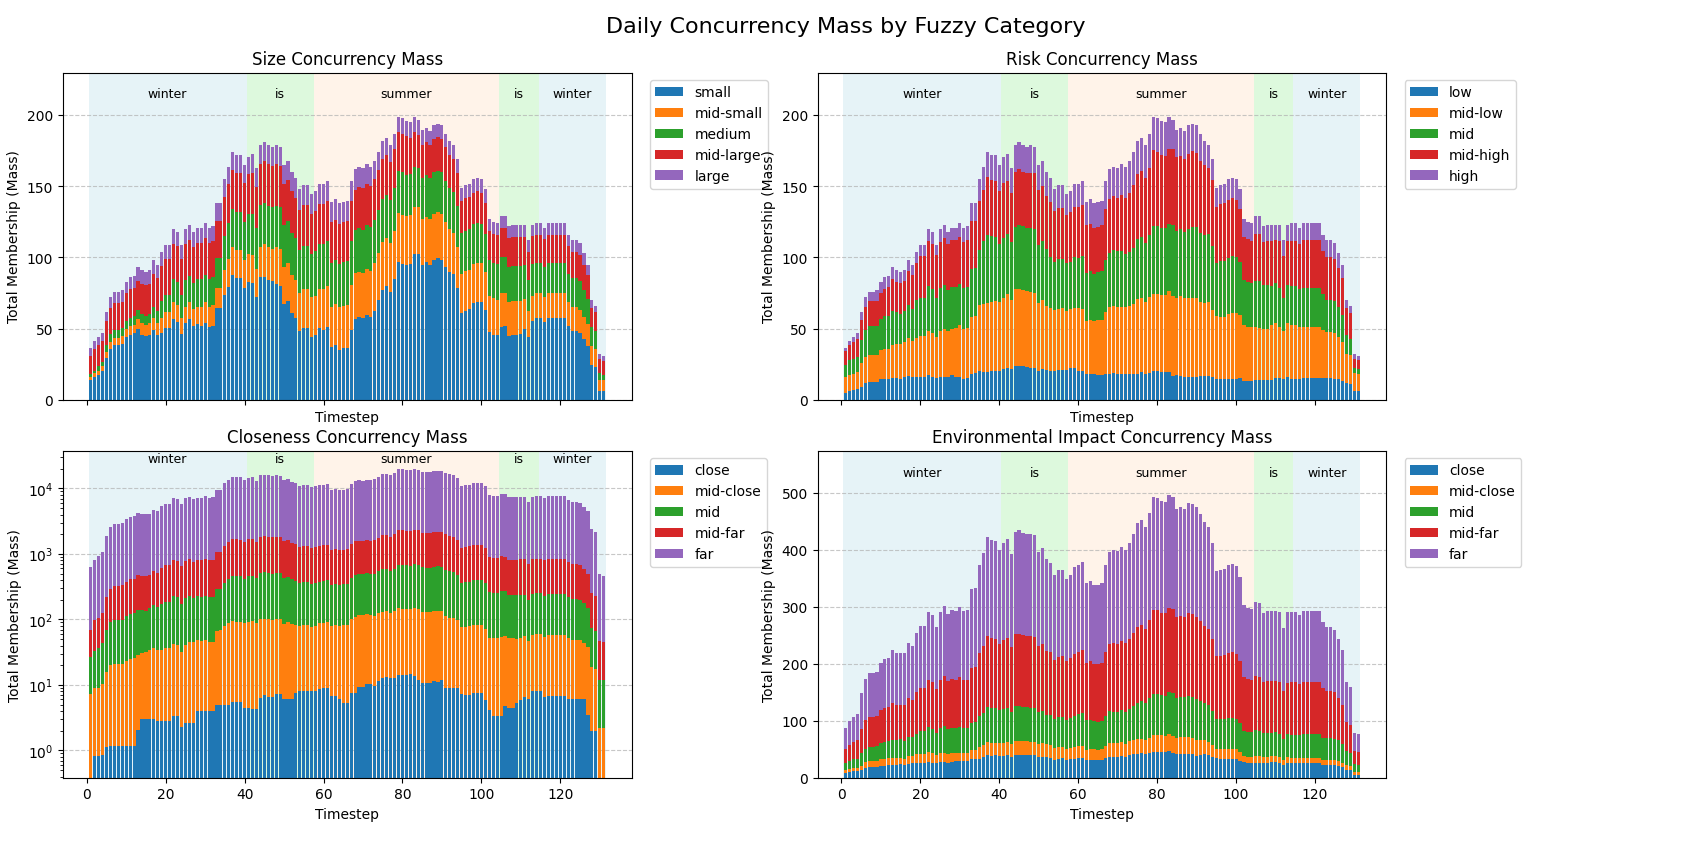
\includegraphics[width=1.07\linewidth]{ch3/figures/Fuzzy_att_concurrency.png}
    \end{adjustwidth}
    \caption{Distribution of daily masses of membership for an example solution throughout the planning horizon.}
    \label{fig:fuzzy_att_concurrency}
\end{figure}

\paragraph{Scoring Uniformity with Entropy.}
For each of the 20 criteria (4 attributes $\times$ 5 fuzzy terms), we possess a daily mass distribution. A desirable schedule should distribute these masses as uniformly as possible over the planning horizon to avoid concentrating risks or resource-heavy tasks. We quantify this uniformity using Shannon's entropy. Given a daily mass vector $M = (m_1, \dots, m_\mathcal{T})$, we first normalize it to a distribution $P = (p_1, \dots, p_\mathcal{T})$, where $p_t = m_t / \sum_{k=1}^\mathcal{T} m_k$. The entropy is then calculated as:
\[
H(P) = - \sum_{t=1}^{\mathcal{T}} p_t \log_2(p_t)
\]
We employ entropy solely as a measure of uniformity, no probabilistic interpretation of the maintenance process is implied. A well-known result from  information theory \cite{Entropy} is that entropy is maximized for a uniform distribution and minimized for one where the mass is concentrated in a single point. Therefore, a higher entropy score corresponds to a more uniform, and thus more desirable, distribution of the fuzzy attribute over time. Final scores are normalized using the entropy of the uniform distribution over $\mathcal{T}$ days which equals $\log_2(\mathcal{T})$.